\section{Discusión y Resultados}
\subsection{Resultados Numéricos: Susceptibilidad, Absorción y Transmisión}
A partir del formalismo desarrollado sobre la matriz de densidad para un sistema atómico de tres niveles en configuración $\Lambda$, la respuesta óptica macroscópica del medio atómico queda gobernada por la susceptibilidad eléctrica compleja $\chi(\Delta_p) = \chi'(\Delta_p) + i\chi''(\Delta_p)$. La simulación numérica así como el resultado obtenido analíticamente para esta expresión revela un comportamiento dual fundamental en el centro de la resonancia de dos fotones ($\Delta_p = 0$ y $\delta = 0$). Por un lado, la componente imaginaria $\chi''$, directamente proporcional al coeficiente de absorción lineal $\alpha(\Delta_p)$, experimenta una caída abrupta. Ésto origina la ventana del EIT, demostrando que la interferencia cuántica destructiva inducida por el campo de acoplamiento de los haces (coupling) suprime la excitación del estado superior $\vert{}3\rangle$.

\begin{figure}[ht]
    \centering
    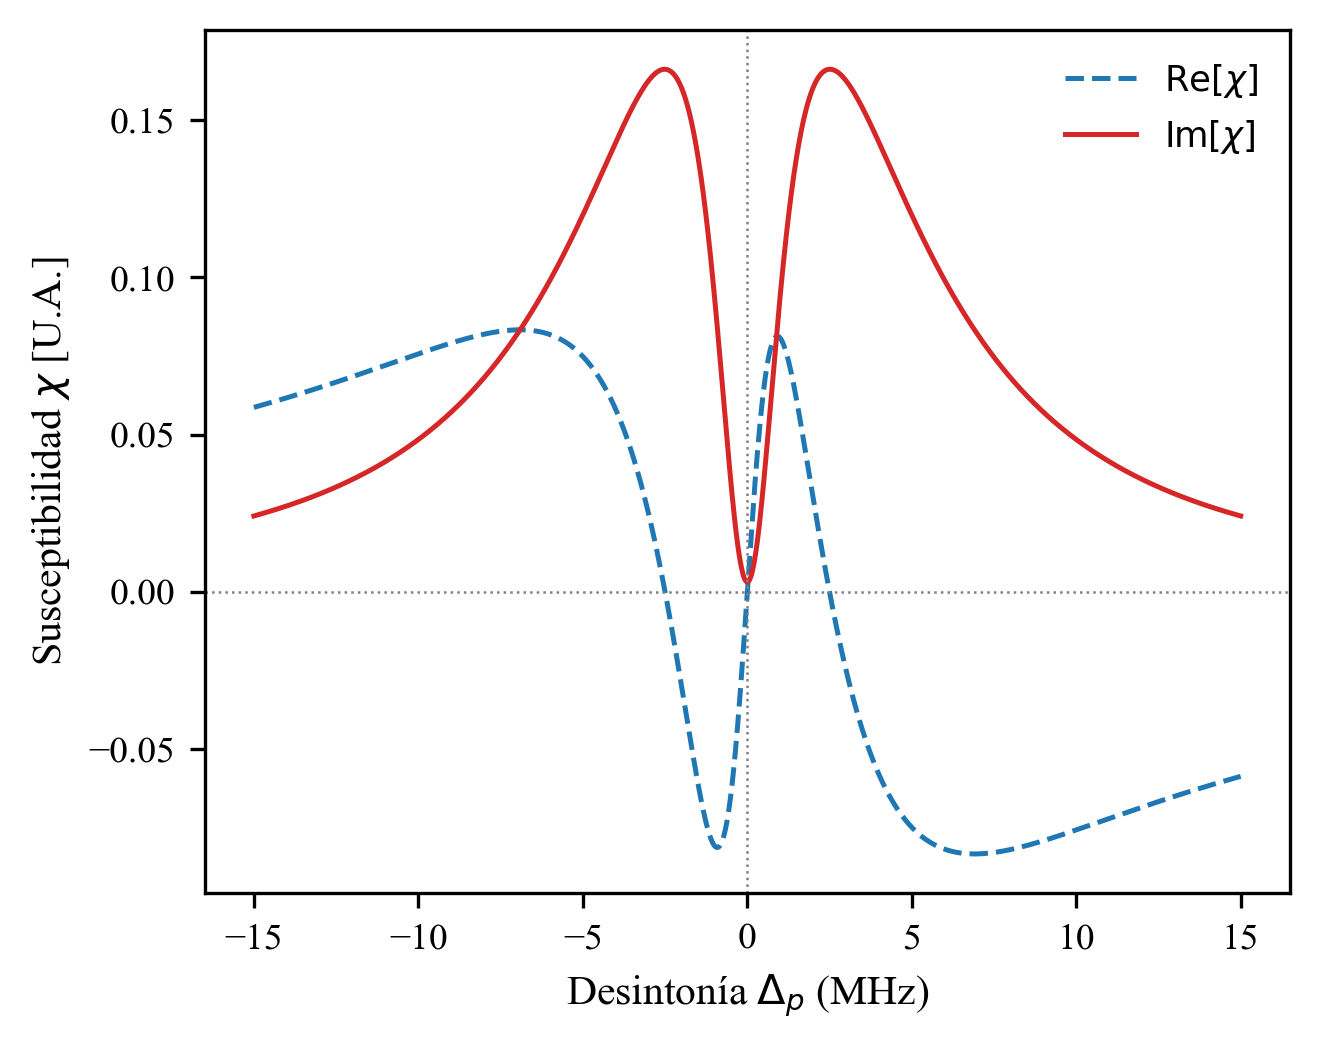
\includegraphics[height = 8cm]{figures/susceptibilidad_eit.png}
    \captionof{figure}{Comportamiento de la parte real (línea punteada) y la parte imaginaria (línea continua) de la susceptibilidad eléctrica $\chi(\Delta_p)$ cerca de resonancia para $\Omega_c = 5\text{ MHz}$. Se observacómo la absorción se va a cero en resonancia de dos fotones ($\delta = 0$); ($\Gamma_{31} = 6.0\text{ MHz}, \Gamma_{21}= 0.02\text{ MHz}, \Delta_c = 0.0 \text{MHz}, k_0 = 1.0 \text{ cm}^{-1}$).}
    \label{fig:eit_susceptibility}
\end{figure}

Por otro lado, la componente real $\chi'$, responsable de la dispersión del medio y relacionada con el índice de refracción $n(\omega) \approx 1 + \frac{1}{2}\chi'$, exhibe una región de dispersión alrededor de la sintonía central, debido a una inflexión. En esta zona, la pendiente de la parte real $(\partial\chi'/\partial\Delta_p)$ adquiere valores positivos muy elevados, lo que modifica drásticamente la velocidad de grupo del pulso óptico de prueba (probe), conduciendo al régimen de luz lenta ($v_g \ll c$).

\subsubsection*{Dependencia del Haz de Control}
\begin{figure}[ht]
    \centering
    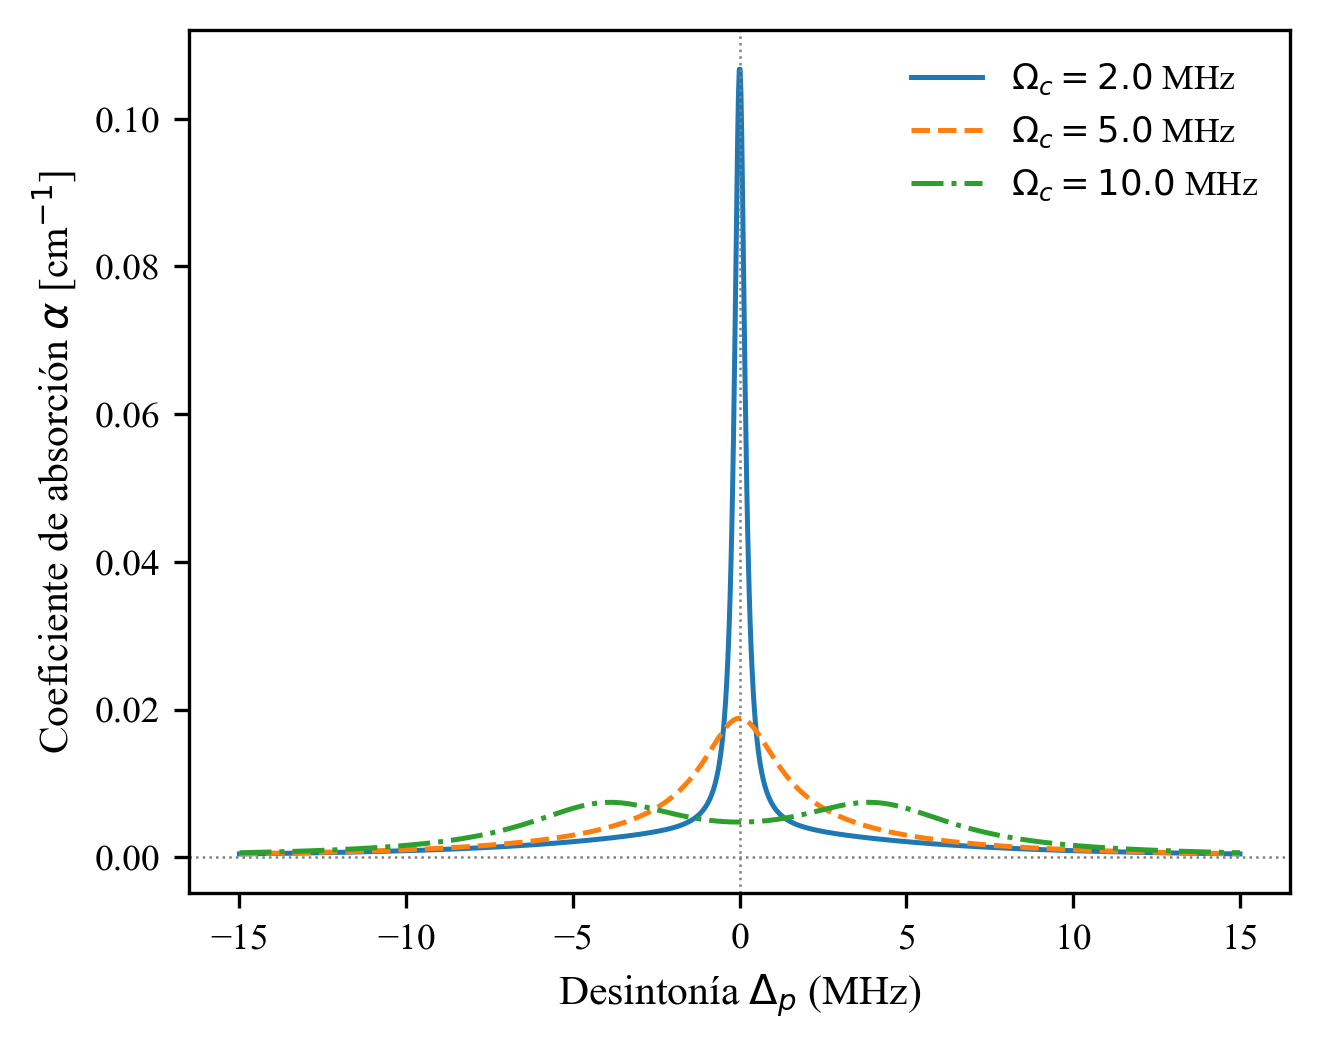
\includegraphics[height = 8cm]{figures/absorcion_eit.png}
    \captionof{figure}{ Perfil del coeficiente de absorción $\alpha(\Delta_p)$ usando diferentes valores para la frecuencia del láser de control ($\Omega_c$). Se observa claramente el pozo de transparencia y cómo la ventana se hace más ancha conforme la potencia del láser de control aumenta; ($\Gamma_{31} = 6.0\text{ MHz}, \Gamma_{21}= 0.02\text{ MHz}, \Delta_c = 0.0 \text{MHz}, k_0 = 1.0 \text{ cm}^{-1}$).}
    \label{fig:eit_absorption}
\end{figure}

Tras analizar el coeficiente de absorción $\alpha(\Delta_p)$ en función de la desintonía del láser de prueba, se observa que la forma de línea resultante difiere notablemente de los perfiles lorentzianos convencionales o de las envolventes simétricas de Voigt de un sistema de dos niveles. En lugar de un máximo central de atenuación, el espectro presenta un mínimo profundo (un dip de transparencia) con dos picos de absorción a los costados. El estudio numérico de este perfil muestra que al variar la frecuencia de Rabi del láser de control ($\Omega_c$) la ventana de transparencia y su ancho varían. En particular, dependen directamente de la intensidad del campo de control $\Omega_{c}$. Conforme se incrementa $\Omega_c$, la anchura a media altura ($\Delta\omega_{\text{EIT}}$) de la ventana de transparencia se ensancha de manera proporcional al cociente $\frac{\vert{}\Omega_c\vert{}^2}{\Gamma_{31}}$, así como un centro de transparencia más elevado.

\subsection*{Transmisión}
Mediante la aplicación de la ley de Beer-Lambert, $\mathcal{T}(\Delta_p) = \exp(-\alpha(\Delta_p) L)$, para una celda atómica de longitud característica $L$, se traduce el coeficiente de absorción en la transmitancia experimental observada en los laboratorios. Los resultados demuestran que el medio pasa de un régimen de opacidad total $(\mathcal{T} \approx 0)$ fuera de resonancia a un estado de alta transmisión óptica $(\mathcal{T} \to 1)$ exactamente en el centro de la ventana EIT.Esta transición limpia y de alta fidelidad confirma la robustez del modelo de tres niveles $\Lambda$ para describir fenómenos coherentes (como lo es el EIT  y la luz lenta) en vapores atómicos.

\begin{figure}[ht]
    \centering
    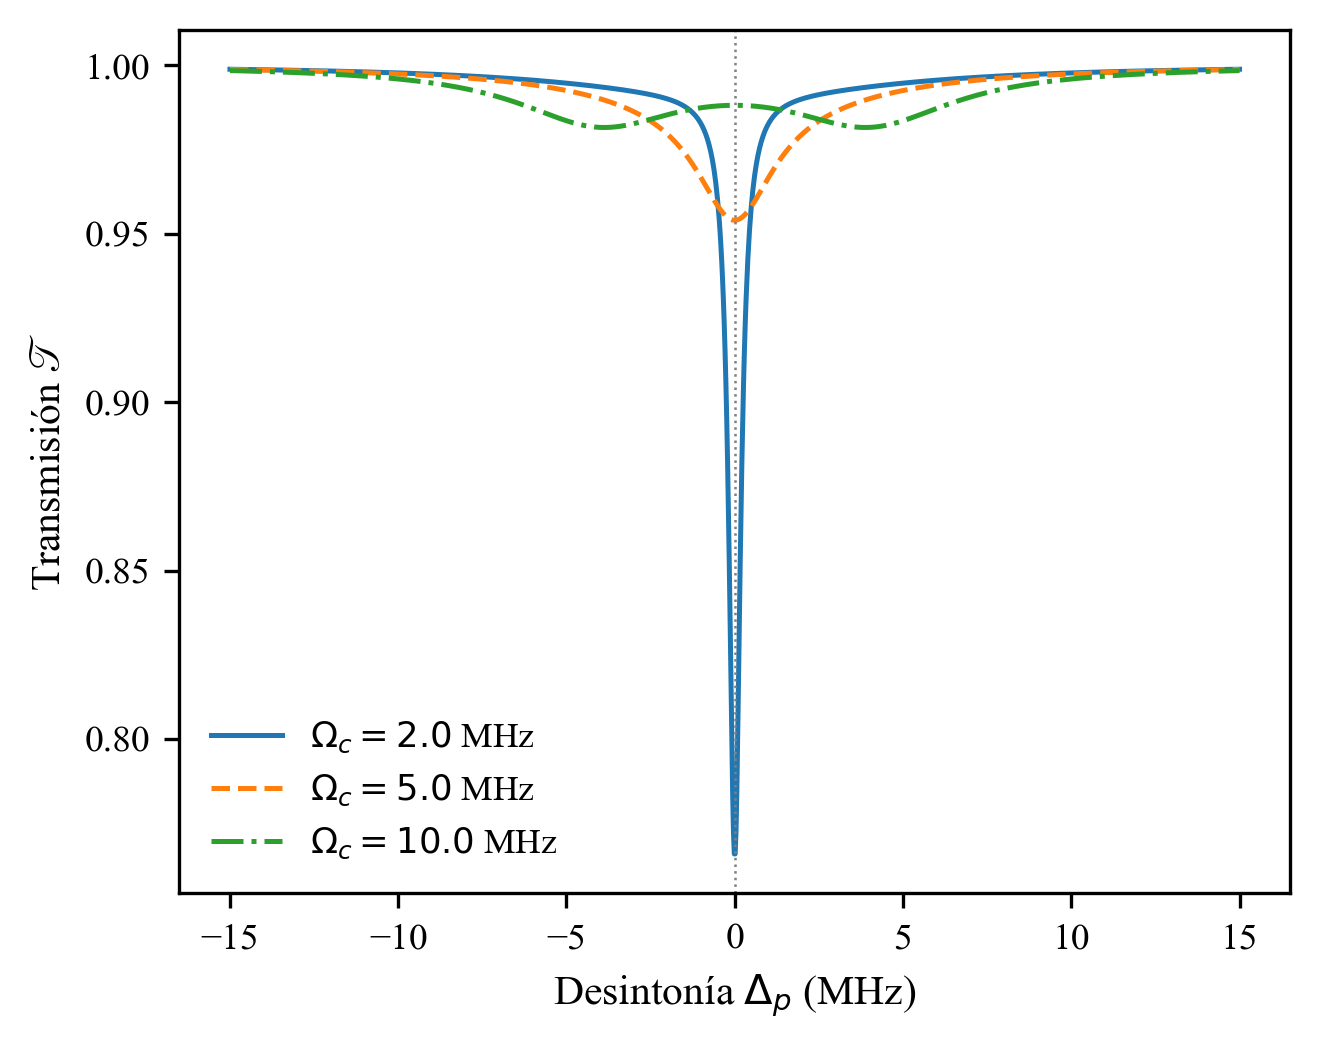
\includegraphics[height = 8cm]{figures/transmision_eit.png}
    \captionof{figure}{Transmisión óptica $\mathcal{T}$ calculada con la ley de Beer-Lambert a través de la celda de vapor atómico. Muestra cómo el medio pasa de bloquear casi toda la luz a alcanzar la transparencia en el centro de la resonancia de dos fotones; ($\Gamma_{31} = 6.0\text{ MHz}, \Gamma_{21}= 0.02\text{ MHz}, \Delta_c = 0.0 \text{MHz}, k_0 = 1.0 \text{ cm}^{-1}, L=2.5 \text{ cm}$).}
    \label{fig:eit_transmission}
\end{figure}

\subsection{Aplicaciones Experimentales y Tecnológicas del EIT}
La Transparencia Inducida Electromagnéticamente (EIT) ha sobrepasado el interés único del estudio de la física cuántica y los sistemas de tres niveles y ha pasado a convertirse en una herramienta tecnológica fundamental para el desarrollo de equipos fotónicos avanzados, procesamiento y almacenamiento de información cuántica así como de metrologóa de alta precisión. Debido a las diversas áreas en las que el EIT forma parte, existen diversas aplicaciones para cada una de ellas.
\subsubsection*{Control de Velocidad de Grupo y Luz Lenta}
Una de las consecuencias más notables del  EIT, como se ha mencionado previamente, es la modificación extema de la velocidad de grupo debido al cambio de la susceptibilidad eléctrica cerca de la ventana de transparencia. Debido a la fuerte dispersión anómala, el índice de refracción de grupo $n_g$ alcanza valores elevados \cite{fleischhauerElectromagneticallyInducedTransparency2005},
\begin{equation}
    n_g = d\dv{k}{\omega} \approx \frac{2\nu_{12}N \mu_{21}}{\hbar \epsilon_0 \Omega_c^2}
\end{equation}
Como resultado la velocidad de grupo de un pulso de luz (en este caso, el haz de prueba) se puede reducir drásticamente a unos pocos metros por segundo en celdas de vapor atómico caliente (como puede ser celdas de Rubidio o Cesio) \cite{kashUltraslowGroupVelocity1999}. 
Gracias a éste control en la velocidad de grupo se pueden comprimir o reprasar pulsos de luz, permitiendo el procesamiento de señales ópticas, líneas de retraso óptico ajustables y el estudio de efectos no lineales debido a la interacción entre fotones bajo arreglos experimentales y aqruitecturas relativamente sencillas.

\subsubsection*{Almacenamiento de Luz y Memorias Cuánticas}
Utilizando la reducción del la velocidad de grupo hasta detener por completo el pulso dentro de la celda, es posible realizar una conversión coherente de la información contenida en el haz de prueba, en particular en una excitación de coherencia de espín atómico. 

Al apagar adiabáticamente el campo de control o acoplamiento (coupling) mientras el pulso óptico se propaga bajo la ventana de EIT, el foton se "congela". En este punto crítico, la energía y la información del fotón no se pierden por absorción debido a la interferencia cuánticca destructiva (el EIT), si no que se transfieren íntegramente a una exitación de coherencia de espín atómico en el estado fundamental hiperfino ($\rho_{21}$). El pulso de luz ha quedado "congelado" en el gas atómico como una onda de espín macroscópica de larga vida.


Para extraer la información almacenada el proceso se invierte de forma temporal. Después de encender el haz de control nuevamente, la coherencia de espín atómico se acopla nuevamente con el campo magnético, la velocidad de grupo acelera hasta alcanzar la habitual en EIT y el puslo de salida conserva de forma idéntica la fase, la forma de onda y las propiedades cuánticas del pulso original.

Ésta técnica de almacenamiento y recuperación de fotones constituye la piedra angular para el desarrollo de redesde  comunicación cuántica y repetidores cuánticos basados en vapores alcalinos.

\subsubsection*{Megnetometría Atómica y Sensores de Alta Sensibilidad}
Los sistemas que implementan EIT o bien el atrapamiento coherente de población (CPT) son altamente sensibles a perturbaciones externas que rompen la degeneración entre los subniveles magnéticos, como pueden ser los campos magnéticos naturals (por ejemplo, el campo magnético terrestre). Debido a que la anchura de la ventana de transparencia para las condiciones experimentales normales es sumamente estrecha (del orden de $\sim \text{kHz}$), variaciones mínimas en el campo magnético inducen desplazamientos Zeeman con altísima precisión en el espectro de transmisión. Ésto ha permitido el diseño de magnetómetros ópticos de bombeo óptico operado a temperatura ambiente en celdas de vapor alcanzando sensibilidades del orden de $\sim \text{fT}$ competitivas con los dispositivos SQUID (Dispositivo de Interferencia Cuántica Superconductora) tradicionales pero sin requerir de sistemas criogénicos.

\subsubsection*{Espectroscopía de Alta Resolución y Estabilización de Láseres}
En el modelado espectroscópica y el ajuste de formas de línea a espectros de absorción, la aparición de picos o caídas angostas que no se ven afectadas por el ensanchamiento Doppler en celdas atómicas calientes proporciona referencias absolutas de frecuencia altamente estables. Éstas caracterísiticas espectrales se utilizan para fijar (lock) las frecuencias de diodos láser a transiciones atómicas hiperfinas específicas de isótopos alcalinos como $^{87}\text{Rb}$ o bien $^{133}\text{Cs}$. 

Éste método garantiza láseres de alta estabilidad en frecuencia para frecuencias específicas en experimentos de óptica cuántica y fotónica, así como en relojes atómicos y sistemas de navegación inercial atómicos.